
\subsection*{Đề thi thử THPTQG Sở GD\&ĐT Sơn La 25--26, Lần 1}

\caulc
\Opensolutionfile{ans}[ans/ans-26-2-SonLa-SoGD-L1-LC]

\begin{ex}%[Thi thử L1 Sở GD Sơn La]%[Phạm Tuấn]%[2D3H1-3]
Mỗi ngày bác Sơn đều đi bộ để rèn luyện sức khỏe. Quãng đường đi bộ mỗi ngày (đơn vị: km) của bác Sơn được cho bởi bảng sau:
\begin{center}
\begin{tabular}{|l|c|c|c|c|c|}
\hline
Quãng đường (km) & $[2{,}7;3{,}0)$ & $[3{,}0;3{,}3)$ & $[3{,}3;3{,}6)$ & $[3{,}6;3{,}9)$ & $[3{,}9;4{,}2)$ \\
\hline
Số ngày & $3$ & $6$ &$ 5$ & $4$ & $2$ \\
\hline
\end{tabular}
\end{center}
Khoảng tứ phân vị của mẫu số liệu ghép nhóm là
\choice
{$0{,}975$}
{$0{,}5$}
{$0{,}9$}
{\True $0{,}575$}
\loigiai{
Ta có $n=20$.\\
Nhóm chứa tứ phân vị thứ nhất là $[3{,}0;3{,}3)$ nên  $Q_{1}=3+\dfrac{5-3}{6} \cdot 0{,}3 = 3{,}1$.\\
Nhóm chứa tứ phân vị thứ ba là $[3,6;3,9)$ nên $Q_{3}=3{,}6+\dfrac{15-14}{4}\cdot 3=3{,}675$. \\
Do đó $\Delta Q=3{,}675-3,1 = 0{,}575$.
}
\end{ex}

\begin{ex}%[Thi thử L1 Sở GD Sơn La]%[Phạm Tuấn]%[2H2N2-3]
Trong không gian $Oxyz$, cho vectơ $\overrightarrow{u}=2\overrightarrow{i}-5\overrightarrow{k}$.  Tọa độ của vectơ là
\choice
{$(2;-5;0)$}
{$(0;2;-5)$}
{$(2;0;5)$}
{\True $(2;0;-5)$}
\loigiai{
Ta có $\overrightarrow{u}=2\overrightarrow{i}+0\overrightarrow{j}-5\overrightarrow{k}\Rightarrow\overrightarrow{u}=(2;0;-5)$.
}
\end{ex}

\begin{ex}%[Thi thử L1 Sở GD Sơn La]%[Phạm Tuấn]%[1D2N3-4]
Cho cấp số nhân $(u_{n})$ có $u_{1}=2$ và $u_{2}=6$. Số hạng của cấp số nhân là
\choice
{$27$}
{\True $54$}
{$162$}
{$11$}
\loigiai{
Ta có $q=\dfrac{u_{2}}{u_{1}}=\dfrac{6}{2}=3$. \\
Do đó $u_{4}=u_{1}\cdot q^{3}=2\cdot3^{3}=54$.
}
\end{ex}

\begin{ex}%[Thi thử L1 Sở GD Sơn La]%[Phạm Tuấn]%[2H2H1-2]
\immini{
Cho hình lập phương $ABCD.A_{1}B_{1}\mathrm{C}_{1}D_{1}$ (tham khảo hình vẽ). Phát biểu nào sau đây đúng?
\choice
{$\overrightarrow{A\mathrm{C}_{1}}=\overrightarrow{AA_{1}}+\overrightarrow{AB}$}
{\True $\overrightarrow{A\mathrm{C}_{1}}=\overrightarrow{AA_{1}}+\overrightarrow{AB}+\overrightarrow{AD}$}
{$\overrightarrow{A\mathrm{C}_{1}}=\overrightarrow{AA_{1}}+\overrightarrow{A_{1}}\overrightarrow{C}$}
{$\overrightarrow{A\mathrm{C}_{1}}=\overrightarrow{AA_{1}}+\overrightarrow{AB}+\overrightarrow{AC}$}
}
{
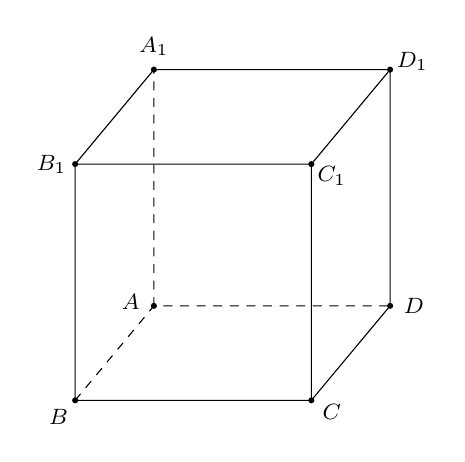
\begin{tikzpicture}[scale=1,font=\footnotesize,line join=round, line cap=round,>=stealth]
\path
(1,1.2) coordinate (A)
(0,0) coordinate (B)
(3,0) coordinate (C)
(4,1.2) coordinate (D)
(1,4.2) coordinate (A_1)
(0,3) coordinate (B_1)
(3,3) coordinate (C_1)
(4,4.2) coordinate (D_1)
;
\draw (B)--(C)--(D)--(D_1)--(C_1)--(B_1)--(A_1)--(D_1) (B)--(B_1) (C)--(C_1);
\draw[dashed] (B)--(A)--(D) (A)--(A_1);
\foreach \x/\g in {A/170, B/225, C/-30, D/0, A_1/90, B_1/180, C_1/-30, D_1/20} 
\fill[black] (\x) circle(1.1pt) + (\g:3mm) node {$\x$};
\end{tikzpicture}
}
\loigiai{
Theo quy tắc hình hộp ta có $\overrightarrow{A\mathrm{C}_{1}}=\overrightarrow{AA_{1}}+\overrightarrow{AB}+\overrightarrow{AD}.$
}
\end{ex}

\begin{ex}%[Thi thử L1 Sở GD Sơn La]%[Phạm Tuấn]%[2D4N2-1]
Cho hàm số $y=f(x)$ thỏa mãn $f(1)=-2,$ $f(2)=1$ và có đạo hàm liên tục trên đoạn $[1; 2]$. Giá trị của tích phân $I=\int\limits _{1}^{2}f'(x)\mathrm{\,d}x$ là
\choice
{$I=-1$}
{$I=2$}
{$I=-3$}
{\True $I=3$}
\loigiai{
Ta có $\displaystyle I=\int\limits _{1}^{2}f'(x) \mathrm{\,d}x=f(x)\big|_{1}^{2}=f(2)-f(1)=1-(-2)=3.$
}
\end{ex}

\begin{ex}%[Thi thử L1 Sở GD Sơn La]%[Phạm Tuấn]%[2D4N1-3]
Họ tất cả các nguyên hàm của hàm số $y=\sin x+\cos x$ là
\choice
{$\int(\sin x+\cos x) \mathrm{\,d}x=\sin x+\cos x+C$}
{$\int(\sin x+\cos x)\mathrm{\,d}x=-\sin x-\cos x+C$}
{$\int(\sin x+\cos x)\mathrm{\,d}x=-\sin x+\cos x+C$}
{\True $\int(\sin x+\cos x)\mathrm{\,d}x=\sin x-\cos x+C.$}
\loigiai{
Ta có $\int (\sin x+\cos x)dx=\sin x- \cos x+C$.
}
\end{ex}

\begin{ex}%[Thi thử L1 Sở GD Sơn La]%[Phạm Tuấn]%[2D1N4-1]
Tiệm cận đứng của đồ thị hàm số $y=\dfrac{2x-1}{x-1}$ là đường thẳng có phương trình 
\choice
{$y=1$}
{\True $x=1$}
{$y=2$}
{$x=2$}
\loigiai{
Ta có $\displaystyle \lim _{x\rightarrow1^{+}}y=+\infty;$ $\displaystyle \lim_{x\rightarrow1^{-}}y=-\infty$ nên tiệm cận đứng của đồ thị hàm số là đường thẳng có phương trình $x=1$.
}
\end{ex}

\begin{ex}%[Thi thử L1 Sở GD Sơn La]%[Phạm Tuấn]%[2H5N1-2]
Cho mặt phẳng $(P):3x-y+z-2=0$. Vectơ nào trong các vectơ dưới đây là một vectơ pháp tuyến của mặt phẳng $(P)$?
\choice
{\True $\overrightarrow{n}=(3;-1;1)$}
{$\overrightarrow{n}=(3;-1;2)$}
{$\overrightarrow{n}=(3;-1;-2)$}
{$\overrightarrow{n}=(3;-1;0)$}
\loigiai{
Mặt phẳng $(P): 3x-y+z-2=0$ có một vectơ pháp tuyến là $\overrightarrow{n}=(3;-1;1).$
}
\end{ex}

\begin{ex}%[Thi thử L1 Sở GD Sơn La]%[Phạm Tuấn]%[1D6N4-2]
Nghiệm của phương trình $\log_{2}(x+1)=3$ là
\choice
{$x=9$}
{\True $x=7$}
{$x=8$}
{$x=5.$}
\loigiai{
Điều kiện  $x>-1$.\\
Ta có  $\log_{2}(x+1)=3\Leftrightarrow x+1=2^{3}\Leftrightarrow x=7$. \\
So với điều kiện ta nhận $x=7$.
}
\end{ex}

\begin{ex}%[Thi thử L1 Sở GD Sơn La]%[Phạm Tuấn]%[1D1N5-3]
Tập nghiệm của phương trình $\cos x=1$ là
\choice
{\True $S=\left \{k2\pi|k\in\mathbb{Z}\right \}$}
{$S=\left \{\dfrac{\pi}{2}+k2\pi|k\in\mathbb{Z}\right \}$}
{$S=\left \{\dfrac{\pi}{2}+k\pi|k\in\mathbb{Z}\right \}$}
{$S=\left \{k\pi|k\in\mathbb{Z}\right \}$}
\loigiai{
Ta có $\cos x=1\Leftrightarrow x=k2\pi(k\in\mathbb{Z})$. \\
Vậy $S=\left \{k2\pi|k\in\mathbb{Z}\right \}$.
}
\end{ex}

\begin{ex}%[Thi thử L1 Sở GD Sơn La]%[Phạm Tuấn]%[1H4N3-2]
\immini{
Cho hình lăng trụ $ABC.A'B'C'$ như hình vẽ. Đường thẳng nào sau đây song song với mặt phẳng $(ACC'A')$?
\choice
{$AA'$}
{\True $BB'$}
{$AC$}
{$AB$}
}
{
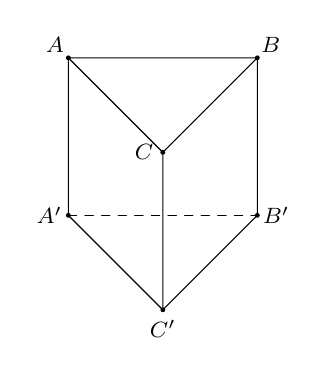
\begin{tikzpicture}[scale=0.8,font=\footnotesize,line join=round, line cap=round,>=stealth]
\path
(0,4) coordinate (A)
(3,4) coordinate (B)
(1.5,2.5) coordinate (C)
(0,1.5) coordinate (A')
(3,1.5) coordinate (B')
(1.5,0) coordinate (C')
;
\draw (A)--(B)--(C)--(A)--(A')--(C')--(B')--(B) (C)--(C');
\draw[dashed] (A')--(B');
\foreach \x/\g in {A/135, B/45, C/180, A'/180, B'/0, C'/-90} 
\fill[black] (\x) circle(1.1pt) + (\g:3mm) node {$\x$};
\end{tikzpicture}
}
\loigiai{
Ta có $\heva{& BB' \notin (ACC'A')\\& BB' \parallel   AA' \\& AA' \subset (ACC'A')}\Rightarrow BB' \parallel (ACC'A')$.
}
\end{ex}

\begin{ex}%[Thi thử L1 Sở GD Sơn La]%[Phạm Tuấn]%[1H8N7-2] 
\immini{
Cho hình chóp $S.ABC$ có $SA \perp (ABC)$, $SA=3$, $\triangle ABC$ vuông cân tại $A$ với $AB=4$.  Thể tích khối chóp $S.ABC$ bằng
\choice
{$48$}
{$16$}
{\True $8$}
{$24$}
}
{
\begin{tikzpicture}[scale=0.8,font=\footnotesize,line join=round, line cap=round,>=stealth]
\path
(0,3.5) coordinate (S)
(0,0) coordinate (A)
(1.5,-2) coordinate (B)
(4.5,0) coordinate (C)
;
\draw (S)--(A)--(B)--(C)--(S)--(B);
\draw[dashed] (A)--(C);
\foreach \x/\g in {S/90, A/180, B/-90, C/0} 
\fill[black] (\x) circle(1.1pt) + (\g:3mm) node {$\x$};
\end{tikzpicture}
}
\loigiai{
Ta có  $S_{\triangle ABC}=\dfrac{1}{2}AB\cdot AC=\dfrac{1}{2}\cdot 4\cdot 4=8$.\\
Do đó $V_{S.ABC}=\dfrac{1}{3}SA\cdot S_{\triangle ABC}=\dfrac{1}{3}\cdot 3\cdot 8=8$.
}
\end{ex}

\Closesolutionfile{ans}


\cauds
\Opensolutionfile{ans}[ans/ans-26-2-SonLa-SoGD-L1-DS]

\begin{ex}%[Thi thử L1 Sở GD Sơn La]%[Phạm Tuấn]%[2D1H5-1]
	\immini{
Cho hàm số $f(x)=x^{3}+3x^{2}-4$.
\choiceTF
{\True Hàm số đã cho có đạo hàm là $f'(x)=3x^{2}+6x$}
{Hàm số đã cho đồng biến trên khoảng $(-1;+\infty)$}
{\True Hàm số đã cho đạt cực đại tại $x=-2$}
{\True Đồ thị của hàm số đã cho có dạng như hình vẽ}
}{
	\begin{tikzpicture}[scale=0.8,font=\footnotesize,line join=round, line cap=round,>=stealth]
		\draw[->] (-4,0)--(2,0) node[below]{$x$};
		\draw[->] (0,-5)--(0,2) node[left]{$y$};
		\clip (-4,-5) rectangle (2,2);
		\draw [smooth,samples=100,domain=-4:2] plot(\x,{(\x)^3+3*(\x)^2-4}) ;
		\draw (-2,0) node[above]{$-2$}  (0,-4) node[below left]{$-4$}   (1,0) node[below right]{$1$}  ;
	\end{tikzpicture}
}
\loigiai{
\begin{itemchoice}
\itemch Ta có  $f'(x)=3x^{2}+6x$.
\itemch Xét tính đồng biến: $f'(x)=3x^{2}+6x$. \\
Ta có $f'(x)>0$ khi $x<-2$ hoặc $x>0$. Hàm số đồng biến trên $(-\infty;-2)$ và $(0;+\infty)$. Không đồng biến trên $(-1;+\infty)$.
\itemch $f'(x)=0\Leftrightarrow3x^{2}+6x=0\Leftrightarrow\hoac{&x=-2\\ &x=0.}$ \\
Bảng biến thiên
\begin{center}

\begin{tikzpicture}
\tkzTabInit[nocadre=false, lgt=1.5, espcl=2]
{$x$ / 0.7 , $y'$ / 0.7 , $y$ / 2}
{$-\infty$ , $-2$ , $0$ , $+\infty$}
\tkzTabLine{ , + , 0 , - , 0 , + , }
\tkzTabVar{-/ $-\infty$ , +/ $0$ , -/ $-4$ , +/ $+\infty$}
\end{tikzpicture}
\end{center}
Bảng biến thiên cho thấy hàm số đã cho đạt cực đại tại $x=-2$.
\itemch  Ta thấy đồ thị phù hợp bảng biến thiên.
\end{itemchoice}
}
\end{ex}

\begin{ex}%[Thi thử L1 Sở GD Sơn La]%[Phạm Tuấn]%[2D5H2-2]
Tại tỉnh $X$, $20\%$ dân số thường xuyên chơi thể thao. Trong số những người thường xuyên chơi thể thao, có $70\%$ người có thể lực tốt. Trong số những người không thường xuyên chơi thể thao, có $15\%$ có thể lực tốt. Chọn ngẫu nhiên một người dân tỉnh $X$.
\choiceTF
{\True Xác suất người đó có thể lực tốt và thường xuyên chơi thể thao là $0{,}14$}
{\True Xác suất người đó có thể lực tốt, biết rằng người đó không thường xuyên chơi thể thao là $0{,}15$}
{Tỉ lệ người có thể lực tốt trong toàn tỉnh $X$ là $36\%$}
{Xác suất người đó thường xuyên chơi thể thao, biết rằng họ có thể lực tốt là $\dfrac{8}{13}$}
\loigiai{
Xét phép thử chọn ngẫu nhiên một người. Gọi $A$ là biến cố: ``Chọn được người thường xuyên chơi thể thao''. \\
$\overline{A}$ là biến cố: ``Chọn được người không thường xuyên chơi thể thao''. \\
Ta có  $\mathrm{P}(A)=0{,}2$; $\mathrm{P}(\overline{A})=0{,}8$. \\
Gọi $B$ là biến cố: ``Chọn được người có thể lực tốt''. \\
Theo bài ra ta có $\mathrm{P}(B|A)=70\%=0{,}7$; $\mathrm{P}(B|\overline{A})=15\%=0{,}15$.
\begin{itemchoice}
\itemch $\mathrm{P}(A\cap B) = \mathrm{P}(A) \mathrm{P}(B|A)=0,2\cdot 0{,}7= 0{,}14$.
\itemch Đề đã cho trực tiếp: $\mathrm{P}(B|\overline{A})=15\%=0{,}15$.
\itemch $\mathrm{P}(B) = \mathrm{P}(A)\mathrm{P}(B|A) + \mathrm{P}(\overline{A})\mathrm{P}(B|\overline{A}) = 0{,}2\cdot 0{,}7+0{,}8\cdot 0{,}15 = 0{,}26$. 
\itemch $\mathrm{P}(A|B)=\dfrac{\mathrm{P}(AB)}{\mathrm{P}(B)}=\dfrac{0{,}14}{0{,}26}=\dfrac{7}{13}$.
\end{itemchoice}
}
\end{ex}

\begin{ex}%[Thi thử L1 Sở GD Sơn La]%[Phạm Tuấn]%[2D1H2-7]
Giả sử lợi nhuận biên (tính bằng triệu đồng) của một sản phẩm được mô hình hoá bằng công thức $P'(x)=-0{,}0008x+10{,}4$. Ở đây $\mathrm{P}(x)$ là lợi nhuận (tính bằng triệu đồng) khi bán được $x$ đơn vị sản phẩm.
\choiceTF
{Lợi nhuận khi bán được $x$ đơn vị sản phẩm được tính bằng công thức $\mathrm{P}(x)=-0{,}0008x^{2}+10{,}4x$}
{\True Lợi nhuận khi bán được $50$ sản phẩm đầu tiên là $519$ triệu đồng}
{Sự thay đổi của lợi nhuận khi doanh số tăng từ $50$ đến $55$ đơn vị sản phẩm là $49{,}79$ triệu đồng}
{Biết sự thay đổi của lợi nhuận khi doanh số tăng từ $50$ lên $a$ đơn vị sản phẩm lớn hơn $517$ triệu đồng, khi đó giá trị nhỏ nhất của $a$ là $100$}
\loigiai{
\begin{itemchoice}
\itemch $P'(x)=-0,0008x+10{,}4$. Lợi nhuận khi bán $x$ đơn vị sản phẩm là $\mathrm{P}(x)=-0{,}0004x^{2}+10{,}4x+C$. Khi không bán sản phẩm nào thì lợi nhuận bằng $0$, tức là $\mathrm{P}(0)=0\Rightarrow C=0$. Vậy $\mathrm{P}(x)=-0{,}0004x^{2}+10{,}4x$.
\itemch Lợi nhuận khi bán $50$ sản phẩm đầu tiên là $\mathrm{P}(50)=-0{,}0004\cdot50^{2}+10{,}4\cdot 50=519$ (triệu đồng).
\itemch Sự thay đổi lợi nhuận khi doanh số tăng từ $50$ đến $55$ đơn vị sản phẩm là $\mathrm{P}(55)-\mathrm{P}(50)=51{,}79$ (triệu đồng).
\itemch Sự thay đổi lợi nhuận khi doanh số tăng từ $50$ lên $a$ đơn vị sản phẩm là 
$$\mathrm{P}(a)-\mathrm{P}(50)=-0{,}0004a^{2}+10{,}4a-519.$$
Theo giả thiết $\mathrm{P}(a)-\mathrm{P}(50)>517 \Leftrightarrow  -0{,}0004a^{2}+10{,}4a-1036>0 \Leftrightarrow 100<a<25900$. \\
Do $a$ nguyên nên giá trị nhỏ nhất của $a$ phải là $101$.
\end{itemchoice}
}
\end{ex}

\begin{ex}%[Thi thử L1 Sở GD Sơn La]%[Phạm Tuấn]%[2H5H3-4]
Một chiếc máy bay thương mại Vietnam Airlines đang bay trên bầu trời theo một đường thẳng từ $D$ đến $E$ có hình chiếu trên mặt đất là đoạn $CB$. Tại vị trí $D$ thì máy bay bay cách mặt đất $9000$ m, tại vị trí $E$ thì máy bay cách mặt đất $12000$ m. Một ra đa được đặt trên mặt đất tại vị trí $O$ cách $C$ khoảng $20000$ m, cách $B$ khoảng $16000$ m và góc $\widehat{BOC}=90^{\circ}$; phạm vi theo dõi của ra đa là $20$ km. Xét hệ trục toạ độ $Oxyz$ (đơn vị trên mỗi trục là $1000$ m) với $O$ là vị trí đặt ra đa, $B$ là điểm thuộc tia $Oy$, $C$ thuộc tia $Ox$.
\begin{center}
\begin{tikzpicture}[x={(-0.5cm,-0.4cm)}, y={(1cm,0cm)}, z={(0cm,1cm)},font=\footnotesize,line join=round, line cap=round,>=stealth]
\path
(0,0,0) coordinate (O)
(4,0,0) coordinate (C)
(0,3.2,0) coordinate (B)
(4,0,1.8) coordinate (D)
(0,3.2,2.4) coordinate (E)
(0,0,1.8) coordinate (Z9)
(0,0,2.4) coordinate (Z12)
;
\draw[->] (0,0,0) -- (6,0,0) node[below] {$x$};
\draw[->] (0,0,0) -- (0,4.5,0) node[right] {$y$};
\draw[->] (0,0,0) -- (0,0,3.5) node[right] {$z$};
\draw (D)--(E);
\draw[dashed] (C)--(D)--(Z9) (B)--(E)--(Z12) (O)--(D) (O)--(E);
\foreach \x/\g in {O/-135, C/-135, B/-90, D/135, E/45} 
\fill[black] (\x) circle(1.1pt) + (\g:3mm) node {};
\draw (B) node[below]{$B(0;16;0)$} (C) node[below right]{$C(20;0;0)$}  (D) node[above left]{$D(20;0;9)$} 
(E) node[above right]{$E(0;16;12)$} (Z9) node[right]{$9$} (Z12) node[left]{$12$} (O) node[below]{$O$};
\end{tikzpicture}
\end{center}
\choiceTF
{Tại $D$, máy bay cách ra đa $21000$ m (làm tròn kết quả đến hàng nghìn theo đơn vị mét)}
{\True Khi máy bay bay đến điểm $I$ thoả mãn $\overrightarrow{DI}=\dfrac{1}{4}\overrightarrow{DE}$ máy bay cách mặt đất $9750$ m}
{\True Trên hành trình bay từ $D$ đến $E$, máy bay sẽ đi qua điểm có toạ độ $\mathrm{P}(16;3{,}2;9{,}6)$}
{Khoảng cách giữa vị trí đầu tiên và vị trí cuối cùng mà máy bay bay trong phạm vi theo dõi của ra đa là $22500$ m (làm tròn đến hàng trăm theo đơn vị mét)}
\loigiai{
\begin{itemchoice}
\itemch Tại $D$, khoảng cách từ máy bay đến ra đa là $OD=\sqrt{20^{2}+0^{2}+9^{2}}=\sqrt{481}\approx 21{,}93$ km $\approx 22000$ m.
\itemch Gọi $I(x;y;z)$. Ta có $\overrightarrow{DI}=\dfrac{1}{4}\overrightarrow{DE}\Rightarrow\begin{cases}x-20=\dfrac{1}{4}(0-20)\\ y-0=\dfrac{1}{4}(16-0)\\ z-9=\dfrac{1}{4}(12-9)\end{cases}\Rightarrow\begin{cases}x=15\\ y=4\\ z=9{,}75.\end{cases}$ \\
Khoảng cách từ máy bay đến mặt đất chính là cao độ $z_{I}=9{,}75$ km $=9750$ m.
\itemch Ta có $\overrightarrow{PD}=(4;-3{,}2;-0{,}6)$ và $\overrightarrow{PE}=(-16;12{,}8;2{,}4) \Rightarrow \overrightarrow{PE}=-4\overrightarrow{PD}$.\\
 Suy ra ba điểm $P$, $D$, $E$ thẳng hàng và điểm $P$ nằm giữa hai điểm $D$ và $E$.
\itemch Đường thẳng $DE$ đi qua $D(20;0;9)$ và có vectơ chỉ phương $\overrightarrow{u}=\overrightarrow{DE}=(-20;16;3)$, $[\overrightarrow{u},\overrightarrow{OD}]=(144;240;-320)$. \\
Khoảng cách từ $O$ đến $DE$ là $d(O,DE)=\dfrac{\left |[\overrightarrow{u},\overrightarrow{OD}]\right |}{\left |\overrightarrow{u}\right |}=\dfrac{\sqrt{144^{2}+240^{2}+(-320)^{2}}}{\sqrt{(-20)^{2}+16^{2}+3^{2}}}=\sqrt{\dfrac{180736}{665}}<20$. \\
Phạm vi theo dõi là mặt cầu tâm $O$, bán kính $R=20$. Đường thẳng $DE$ cắt mặt cầu tại hai điểm $A$, $B$. \\
Khoảng cách cần tìm là $AB=2\sqrt{R^{2}-d^{2}}=2\sqrt{20^{2}-\dfrac{180736}{665}}\approx 22{,}6465$ km $\approx 22600$ m.
\end{itemchoice}
}
\end{ex}

\Closesolutionfile{ans}

\caukq
\Opensolutionfile{ans}[ans/ans-26-2-SonLa-SoGD-L1-KQ]

\begin{ex}%[Thi thử L1 Sở GD Sơn La]%[Phạm Tuấn]%[1D9V2-4]
Trong một cuộc thi đấu Robotics, sân đấu được thiết kế dạng lưới ô vuông như hình vẽ. Các robot xuất phát từ vị trí điểm $A$, di chuyển ngẫu nhiên theo cạnh của các ô vuông theo hướng xuống dưới hoặc sang phải đến vị trí điểm $B$. Tính xác suất robot đi từ $A$ đến $B$ mà không đi qua cả $M$ và $N$ (kết quả làm tròn đến hàng phần trăm).
\begin{center}
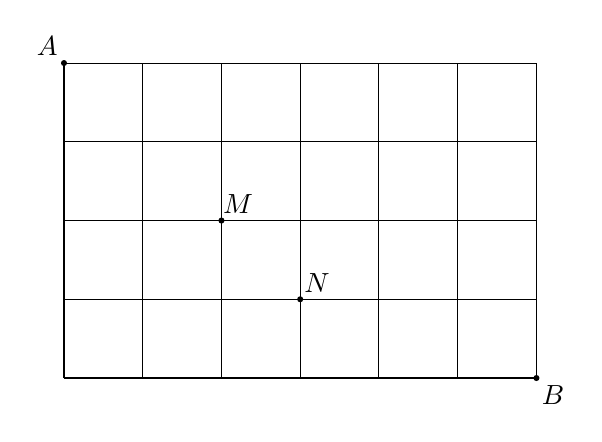
\begin{tikzpicture}
\path
(0,4) coordinate (A)
(6,0) coordinate (B)
(2,2) coordinate (M)
(3,1) coordinate (N)
;
\draw (0,0) grid (6,4);
\foreach \x/\g in {A/135, B/-45, M/45, N/45} 
\fill[black] (\x) circle(1.1pt) + (\g:3mm) node {$\x$};
\end{tikzpicture}
\end{center}
\par\shortans{$0,42$}
\loigiai{
Ta coi việc robot đi qua một cạnh của ô vuông nhỏ là một bước. Robot xuất phát từ $A$ muốn đến $B$ phải đi chuyển sang ngang $6$ bước và xuống dưới $4$ bước, tổng là $10$ bước. Vì vậy, số cách di chuyển của robot từ $A$ đến $B$ là $\mathrm{C}_{10}^{6}\cdot \mathrm{C}_{4}^{4}=\mathrm{C}_{10}^{6}$.\\
Gọi $E$ là biến cố: “Robot đi từ $A$ đến $B$ mà phải đi qua $M$”. $F$ là biến cố: “Robot đi từ $A$ đến $B$ mà phải đi qua $N$”.\\
Suy ra $E \cap F$ là biến cố: “Robot đi từ $A$ đến $B$ mà phải đi qua cả $M$ và $N$”. \\
$E \cup F$ là biến cố: “Robot đi từ $A$ đến $B$ mà phải đi qua ít nhất một trong hai điểm $M$ và $N$”. Khi đó biến cố: ``Robot đi từ $A$ đến $B$ mà không đi qua cả $M$ và $N$'' là biến cố đối của biến cố $E \cup F$.
\begin{itemize}
\item Đi từ $A$ đến $M$ cần $2$ bước sang ngang và $2$ bước xuống dưới, tổng là $4$ bước nên số cách đi $\mathrm{C}_{4}^{2}$.
\item Đi từ $M$ đến $B$ cần $4$ bước sang ngang và $2$ bước xuống dưới, tổng là $6$ bước nên số cách đi $\mathrm{C}_{6}^{4}$.
\end{itemize}
Ta có $n(E)=\mathrm{C}_{4}^{2}\cdot \mathrm{C}_{6}^{4}$;  $n(F)=\mathrm{C}_{6}^{3}\cdot \mathrm{C}_{4}^{3}$, $n(E \cap F)=\mathrm{C}_{4}^{2}\cdot \mathrm{C}_{2}^{1}\cdot \mathrm{C}_{4}^{3}$.\\
Suy ra $\mathrm{P}(E\cup F)=\dfrac{n(E)+n(F)-n(E \cap F)}{n(\Omega)}=\dfrac{\mathrm{C}_{4}^{2}\cdot \mathrm{C}_{6}^{4}+\mathrm{C}_{6}^{3}\cdot \mathrm{C}_{4}^{3}-\mathrm{C}_{4}^{2}\cdot \mathrm{C}_{2}^{1}\cdot \mathrm{C}_{4}^{3}}{\mathrm{C}_{10}^{6}}=\dfrac{61}{105}$.  \\
Xác suất robot đi từ $A$ đến $B$ mà không đi qua cả $M$ và $N$ là $1-\mathrm{P}(E\cup F)=\dfrac{44}{105}\approx 0{,}42$.
}
\end{ex}

\begin{ex}%[Thi thử L1 Sở GD Sơn La]%[Phạm Tuấn]%[1H8V5-3
Cho hình chóp $S.ABCD$ có đáy $ABCD$ là hình thoi tâm $O$, cạnh bằng $1$, góc $\widehat{ABC}=60^{\circ}$. Biết rằng $SO \perp (ABCD)$, $SO=\dfrac{3}{2}$. Tính khoảng cách từ $A$ đến mặt phẳng $(SCD)$ (không làm tròn kết quả ở các bước trung gian, làm tròn kết quả ở bước cuối cùng đến hàng phần trăm).
\par\shortans{$0,83$}
\loigiai{
\begin{center}
\begin{tikzpicture}
\path
(0,0) coordinate (B)
(4,0) coordinate (C)
(1.4,1.5) coordinate (A)
($(A)+(C)-(B)$) coordinate (D)
(2.6,0.75) coordinate (O)
(2.6,4.5) coordinate (S)
($(C)!0.5!(D)$) coordinate (H)
($(S)!0.5!(H)$) coordinate (K)
;
\draw (S)--(B)--(C)--(D)--(S)--(C) (S)--(H);
\draw[dashed] (S)--(A)--(B) (A)--(D) (A)--(C) (B)--(D) (S)--(O)--(H) (O)--(K);
\foreach \x/\g in {S/90, A/180, B/-135, C/-45, D/0, O/-90, H/0, K/0} 
\fill[black] (\x) circle(1.1pt) + (\g:3mm) node {$\x$};
\end{tikzpicture}
\end{center}
Đáy $ABCD$ là hình thoi tâm $O$ cạnh bằng $1$, góc $\widehat{ABC}=60^{\circ}$ nên tam giác $ABC$ là tam giác đều cạnh $1$. Suy ra đường chéo $AC=1\Rightarrow AO=OC=\dfrac{1}{2}$. Trong tam giác $ABC$ đều, đường cao từ $B$ (cũng là một nửa đường chéo $BD$) có độ dài $OB=\dfrac{\sqrt{3}}{2}\Rightarrow OD=\dfrac{\sqrt{3}}{2}$. \\
Vì $O$ là trung điểm của $AC$ nên khoảng cách từ $A$ đến $(SCD)$ gấp đôi khoảng cách từ $O$ đến $(SCD)$, tức là $d(A,(SCD))=2d(O,(SCD))$.\\
Kẻ $OH \perp CD$ tại $H$. Do $SO \perp (ABCD)$ nên $SO \perp CD$. Từ đó suy ra $CD\perp(SOH)\Rightarrow(SCD) \perp (SOH)$.\\ Mặt phẳng $(SCD)$ và $(SOH)$ cắt nhau theo giao tuyến $SH$. Trong mặt phẳng $(SOH)$, kẻ $OK \perp SH$ tại $K$. Khi đó $OK \perp (SCD)$, suy ra $d(O,(SCD))=OK$.\\
Xét tam giác vuông $OCD$ tại $O$, đường cao $OH$ thỏa mãn 
\[
\dfrac{1}{OH^{2}}=\dfrac{1}{OC^{2}}+\dfrac{1}{OD^{2}}=\dfrac{1}{\left (\dfrac{1}{2}\right )^{2}}+\dfrac{1}{\left (\dfrac{\sqrt{3}}{2}\right )^{2}}=\dfrac{16}{3}.
\]
Xét tam giác vuông $SOH$ tại $O$, đường cao $OK$ thỏa mãn 
$$\dfrac{1}{OK^{2}}=\dfrac{1}{SO^{2}}+\dfrac{1}{OH^{2}}=\dfrac{1}{\left (\dfrac{3}{2}\right )^{2}}+\dfrac{16}{3}=\dfrac{52}{9}.$$
Suy ra $OK=\dfrac{3}{\sqrt{52}}=\dfrac{3}{2\sqrt{13}}$. \\
Khoảng cách cần tìm là $d(A,(SCD))=2OK=2\cdot\dfrac{3}{2\sqrt{13}}=\dfrac{3}{\sqrt{13}}\approx 0{,}83$.
}
\end{ex}

\begin{ex}%[Thi thử L1 Sở GD Sơn La]%[Phạm Tuấn]%[2D1V3-6]
Một nhà địa chất học đang ở địa điểm $A$ trên sa mạc. Anh ta muốn đến điểm $B$ (cũng ở trên sa mạc) và cách $A$ một khoảng bằng $70$ km. Trong sa mạc, xe anh ta chỉ có thể di chuyển với vận tốc $30$ km. Nhà địa chất phải đến được điểm $B$ sau $2$ giờ, vì vậy nếu anh ta đi thẳng từ $A$ đến $B$ sẽ không thể đến đúng giờ được. Rất may, có một con đường nhựa song song với đường nối $A$ và $B$ và cách $AB$ một đoạn $10$ km (tham khảo hình vẽ). Trên đường nhựa đó, xe nhà địa chất có thể di chuyển với vận tốc $50$ km. Thời gian ngắn nhất để nhà địa chất di chuyển từ $A$ đến $B$ là bao nhiêu phút?
\begin{center}
\begin{tikzpicture}
\path
(0,3) coordinate (A)
(8,3) coordinate (B)
(2.5,0) coordinate (C)
(5.5,0) coordinate (D)
;
\draw (-1,0)--(9,0) (A)--(C) (B)--(D) (-0.5,0)--(-0.5,3) (-0.6,0)--(-0.4,0) (-0.6,3)--(-0.4,3);
\draw[dashed] (A)--(B);
\foreach \x/\g in {A/90, B/90, C/-90, D/-90} 
\fill[black] (\x) circle(1.1pt) + (\g:3mm) node {$\x$};

\node[left] at (-0.5, 1.5) {10km};
\node at (4, 1.5) {Sa mạc};
\node[below] at (4, -0.2) {Đường nhựa};
\end{tikzpicture}
\end{center}
\par\shortans{$116$}
\loigiai{
Gọi $H$, $K$ lần lượt là hình chiếu của $A$, $B$ lên đường thẳng $CD$. Khi đó gọi $HC=x(0<x<70)$ và $DK=y(0<y<70)$.\\
Quãng đường đi từ $A$ đến $C$ là $AC=\sqrt{10^{2}+x^{2}}$ (km), thời gian đi từ $A$ đến $C$ là $\dfrac{\sqrt{10^{2}+x^{2}}}{30}$ (giờ). \\
Quãng đường đi từ $D$ đến $B$ là $DB=\sqrt{10^{2}+y^{2}}$ (km), thời gian đi từ $D$ đến $B$ là $\dfrac{\sqrt{10^{2}+y^{2}}}{30}$ (giờ). \\
Quãng đường đi $C$ đến $D$ là $CD=70-(x+y)$ (km), thời gian đi từ $C$ đến $D$ là $\dfrac{70-(x+y)}{50}$ (giờ).\\
Thời gian mà nhà địa chất học đi từ $A$ đến $C$, đến $D$ rồi đến $B$ là 
\[
T=\dfrac{\sqrt{10^{2}+x^{2}}}{30}+\dfrac{\sqrt{10^{2}+y^{2}}}{30}+\dfrac{70-(x+y)}{50}=\left(\dfrac{\sqrt{10^{2}+x^{2}}}{30}+\dfrac{35-x}{50}\right)+\left(\dfrac{\sqrt{10^{2}+y^{2}}}{30}+\dfrac{35-y}{50}\right).
\]
Đặt $f(u)=\dfrac{\sqrt{10^{2}+u^{2}}}{30}+\dfrac{35-u}{50}$ với $0<u<70$. Ta có $f'(u)=\dfrac{u}{30\sqrt{10^{2}+u^{2}}}-\dfrac{1}{50}$.\\
Cho $f'(u)=0\Leftrightarrow 50u=30\sqrt{10^{2}+u^{2}}\Leftrightarrow \sqrt{10^{2}+u^{2}}=\dfrac{5u}{3}\Leftrightarrow u=\dfrac{15}{2}$.\\
Lập bảng biến thiên ta có $\min_{u\in(0,70)}f(u)=f\left(\dfrac{15}{2}\right)=\dfrac{29}{30}$.\\
Dấu $``=''$ xảy ra khi $x=y=\dfrac{15}{2}$. Suy ra $T=f(x)+f(y)\ge \dfrac{29}{30}+\dfrac{29}{30}=\dfrac{29}{15}$.\\
Vậy thời gian ngắn nhất để nhà địa chất di chuyển từ $A$ đến $B$ là $\dfrac{29}{15}\cdot60=116$ phút.
}
\end{ex}

\begin{ex}%[Thi thử L1 Sở GD Sơn La]%[Phạm Tuấn]%[0D2H2-3]
Trong một cuộc thi làm bánh, mỗi đội chỉ được sử dụng tối đa $6$ kg bột mì và $4$ kg đậu để làm ra bánh loại I và bánh loại II. Để làm ra một chiếc bánh loại I cần $0{,}06$ kg bột mì và $0{,}08$ kg đậu, để làm ra một chiếc bánh loại II cần $0{,}08$ kg bột mì và $0{,}04$ kg đậu. Mỗi chiếc bánh loại I được $8$ điểm, mỗi chiếc bánh loại II được $10$ điểm. Số điểm tối đa có thể đạt được của mỗi đội bằng bao nhiêu?
\par\shortans{$760$}
\loigiai{
Gọi $x$ là số bánh loại I $(x\ge0,x\in\mathbb{Z})$. Gọi $y$ là số bánh loại II $(y\ge 0,y\in\mathbb{Z})$. \\
Số điểm đạt được là $F(x,y)=8x+10y$. \\
Hệ điều kiện: $\heva{&x\ge0\\ &y\ge 0\\ &0{,}06x+0{,}08y\le6\\ &0{,}08x+0{,}04y\le 4}\Leftrightarrow\heva{&x\ge 0\\ &y\ge 0\\ &3x+4y\le300\\ &2x+y\le100.}$ \\
Tập nghiệm của hệ bất phương trình là miền tứ giác $OABC$, với $O(0;0)$, $A(50;0)$, $B(20;60)$, $C(0;75)$. 
\begin{center}
\begin{tikzpicture}[>=stealth, scale=0.5,]
    \fill[pattern=north east lines, even odd rule]
        (-1.5,-1.5) rectangle (11.5,11.5)
        (0,0) -- (5,0) -- (2,6) -- (0,7.5) -- cycle;

    
    \draw[->, thick] (-1.5,0) -- (11.5,0) node[below] {$x$};
    \draw[->, thick] (0,-1.5) -- (0,11.5) node[left] {$y$};
    \node[below left] at (0,0) {$O$};

    
    \foreach \x in {1,2,3,4,5,6,7,8,9,10} {
        \draw (\x,0.1) -- (\x,-0.1);
    }
    \foreach \y in {1,2,3,4,5,6,7,8,9,10} {
        \draw (0.1,\y) -- (-0.1,\y);
    }

    \node[below] at (2,0) {$20$};
    \node[below] at (5,0) {$50$};
    \node[below] at (10,0) {$100$};
    
    \node[left] at (0,6) {$60$};
    \node[left] at (0,7.5) {$75$};
    \node[left] at (0,10) {$100$};
    \draw[thick] (-1.333, 8.5) -- (11.333, -1);
    \draw[thick] (-0.5, 11) -- (5.5, -1);
    \fill (0,0) circle (2pt);
    \fill (5,0) circle (2pt) node[above right] {$A$};
    \fill (2,6) circle (2pt) node[above right] {$B$};
    \fill (0,7.5) circle (2pt) node[above right] {$C$};
    \draw[dashed] (2,0) -- (2,6) -- (0,6);
\end{tikzpicture}
\end{center}
\begin{itemize}
\item Tại $O(0;0)$: $F=8 \cdot 0 +10 \cdot 0=0$ (điểm).
\item Tại $A(50;0)$: $F=8 \cdot  50+10 \cdot 0=400$ (điểm). 
\item Tại $B(20;60)$: $F=8 \cdot  20+10 \cdot 60=760$ (điểm).
\item Tại $C(0;75)$: $F=8 \cdot 0 +10 \cdot  75=750$ (điểm).
\end{itemize}
Vậy số điểm tối đa có thể đạt được của mỗi đội là $760$ điểm khi làm $20$ cái bánh loại I và $60$ cái bánh loại II.
}
\end{ex}

\begin{ex}%[Thi thử L1 Sở GD Sơn La]%[Phạm Tuấn]%[2D4H3-3]
Từ một quả cầu bằng đá trắng bán kính bằng $1$ dm người ta khoan rút lõi ngay “chính giữa” quả cầu (trục đối xứng của lõi và quả cầu trùng nhau) như hình minh họa, đường kính lõi là $1$ dm. Thể tích còn lại của quả cầu bằng bao nhiêu $\text{dm}^{3}$? (không làm tròn kết quả ở các bước trung gian, làm tròn kết quả ở bước cuối cùng đến hàng phần trăm).
\begin{center}
\begin{minipage}[t]{0.45\textwidth}
\begin{center}
\begin{tikzpicture}[scale=0.5]
\draw (0,0) circle ({sqrt(29)}) ;
\draw[thick] (2,5) arc (0:-180:2 cm and 0.2 cm);
\draw[dashed] (2,5) arc (0:180:2 cm and 0.2 cm);
\draw[thick] (2,-5) arc (0:-180:2 cm and 0.2 cm);
\draw[dashed] (2,-5) arc (0:180:2 cm and 0.2 cm);
\draw[dashed] (-2,5)--(-2,-5)  (2,5)--(2,-5);
\draw (0,-6) node[]{Quả cầu đá} ;
\end{tikzpicture}
\end{center}
\end{minipage}
\begin{minipage}[t]{0.5\textwidth}
\begin{center}
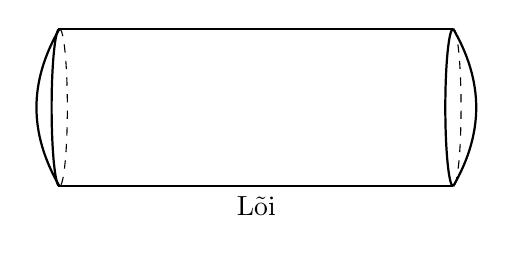
\begin{tikzpicture}[scale=0.5]
\begin{scope}[rotate=90]
\draw[thick] (2,5) arc (0:180:2 cm and 0.2 cm);
\draw[dashed] (2,5) arc (0:-180:2 cm and 0.2 cm);
\draw[thick] (2,-5) arc (0:180:2 cm and 0.2 cm);
\draw[dashed] (2,-5) arc (0:-180:2 cm and 0.2 cm);
\draw[thick] (-2,5)--(-2,-5)  (2,5)--(2,-5);
\draw [thick] (-2,5) to [bend left] (2,5);
\draw [thick] (-2,-5) to [bend right] (2,-5);
\end{scope}
\draw (0,-2.5) node[]{Lõi} ;
\end{tikzpicture}
\end{center}
\end{minipage}
\end{center}
\par\shortans{$2,72$}
\loigiai{
Thể tích quả cầu đá ban đầu là  $V=\dfrac{4}{3}\pi\cdot1^{3}=\dfrac{4}{3}\pi$. \\
Thể tích phần lõi bằng tổng thể tích $V_{1}$ của khối trụ có bán kính đáy $\dfrac{1}{2}$ dm, chiều cao $h=2\sqrt{1^{2}-\left(\dfrac{1}{2}\right)^{2}}=\sqrt{3}$ và thể tích $V_{2}$ của hai chỏm cầu có chiều cao $\dfrac{2-\sqrt{3}}{2}$ dm của khối cầu ban đầu.\\
Suy ra thể tích phần còn lại của quả cầu là
\[
V_{3}=V-V_{1}-V_{2}=\dfrac{4}{3}\pi-\pi\left(\dfrac{1}{2}\right)^{2}\cdot\sqrt{3}-2\cdot\dfrac{1}{3}\cdot\pi\cdot\left(\dfrac{2-\sqrt{3}}{2}\right)^{2}\left(3\cdot1-\dfrac{2-\sqrt{3}}{2}\right)\approx 2,72.
\]
\textbf{Chú ý}: Thể tích chỏm cầu bán kính $R$, chiều cao $h$ được tính theo công thức 
$$V=\frac{\pi h^2}{3}(3 R-h).$$
}
\end{ex}

\begin{ex}%[Thi thử L1 Sở GD Sơn La]%[Phạm Tuấn]%[0D8V2-7]
Cho hình vẽ dưới đây gồm $4$ tam giác. Người ta chọn $3$ số phân biệt từ tập hợp $S=\{1;2;...;26\}$ để xếp vào $3$ tam giác ở $3$ góc. Sau đó, tính tổng bình phương của $3$ số đó rồi ghi kết quả vào tam giác còn lại ở giữa. Hỏi có bao nhiêu cách xếp sao cho số ghi ở tam giác giữa là một số chia hết cho $5$?
\begin{center}
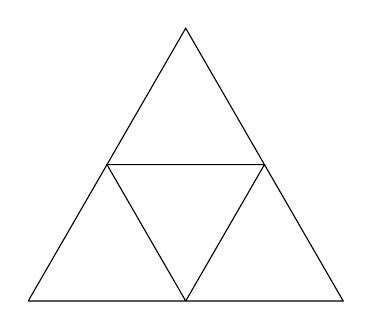
\begin{tikzpicture}
\path
(0,0) coordinate (A)
(4,0) coordinate (B)
(2,3.4641) coordinate (C)
(2,0) coordinate (M)
(3,1.732) coordinate (N)
(1,1.732) coordinate (P)
;
\draw (A)--(B)--(C)--(A) (M)--(N)--(P)--(M);
\foreach \x/\g in {} 
\fill[black] (\x) circle(1.1pt) + (\g:3mm) node {$\x$};
\end{tikzpicture}
\end{center}
\par\shortans{$3360$}
\loigiai{
Một số nếu chia hết cho $5$ thì bình phương của nó sẽ chia hết cho $5$, nếu chia cho $5$ dư $1$ thì bình phương của nó chia $5$ dư $1$, nếu chia $5$ dư $2$ thì bình phương của nó chia $5$ dư $4$, nếu chia $5$ dư $3$ thì bình phương của nó chia $5$ dư $4$, nếu chia $5$ dư $4$ thì bình phương của nó chia $5$ dư $1$. Ta chia các số thuộc tập $S$ thành các nhóm sau: 
\begin{itemize}
\item Nhóm 1 gồm $5$ số có bình phương chia hết cho $5$. 
\item Nhóm 2 gồm $11$ số có bình phương chia $5$ dư $1$. 
\item Nhóm 3 gồm $10$ số có bình phương chia $5$ dư $4$. 
\end{itemize}
Để tổng bình phương của $3$ số được chọn chia hết cho $5$ ta xét các trường hợp sau: \\
\textbf{Trường hợp 1}: Chọn $3$ số thuộc nhóm 1 thì có $\mathrm{C}_{5}^{3}=10$ cách.\\
\textbf{Trường hợp 2}: Chọn $1$ số thuộc nhóm 1, $1$ số thuộc nhóm 2, $1$ số thuộc nhóm 3 thì có $5\cdot11\cdot10 = 550$ cách. \\
Vậy có $550+10=560$ cách chọn được $3$ số có tổng các bình phương của chúng chia hết cho $5$. \\
Suy ra số cách xếp sao cho số ghi ở tam giác giữa là một số chia hết cho $5$ là  $560\cdot3! = 3360$ cách.
}
\end{ex}
\Closesolutionfile{ans}
%\indapan{6}{ans/ans-26-2-SonLa--SoGD-L1-LC}
%\indapan{4}{ans/ans-26-2-SonLa-SoGD-L1-DS}
%\indapan{6}{ans/ans-26-2-SonLa-SoGD-L1-KQ}
